\begin{letter}{8}
\begin{header}
\from{Schr\"odinger}
\to{Pauli}
\date{1920/07/12}
\location{Jena}

\makeheader

\end{header}

Dear Herr Pauli!

Many thanks for your letter. I am glad to hear that are paying attention to the poor, long-neglected magnetism and have put beautiful results about it within reach, and also glad that we have come to an understanding, since it would be madness to work in parallel and on top of one another now, when the field \WTF{in Modellangelegenheiten} is truly large enough to, on the contrary, to make the most parsimonious \textit{division of labor} a pressing demand. Since the matter however has not stopped being very compellingly interesting to me, I would be very thankful to you if you would be able to make it possible for me  to get a proof of your relevant paper as soon as possible — in the present \?{conditions of publication}{Publikationsverhältnissen} it otherwise takes far too long to be able to eventually include further reflections, and life is short.

I am very curious on your diamagnetic note. Namely it seems to me that e.g. in helium the Bohr orbits are not at all sufficient for explaining the relatively strong diamagnetism ($\kappa = -11\cdot 10^{-9}$), even if it is not partially obscured by a (of course very weak) orientation effect. So the diamagnetism might be in part a nuclear effect, which would be quite interesting — it would then, assuming sufficiently precise measurement, provide alongside gravitation and radioactivity a third means of distinguishing isotopes.

That the \WTF{Kreiselmodell} should \textit{not} give the Curie law would astonish me, and I cannot quite believe this result, that you yourself only expressed with great reservations. — For me, a great difficulty in the \textit{Kreiselmodell} lies in the following. I will call the motion \textit{without} an $H$-field a \WTF{Thermopräzession}, the aperture angles are then "quantized" in the well-known manner. The moment \textit{in the direction of the field}\footnote{therefore the cosine of the field direction-axis of thermal precession angle.} however should, according to Epstein (Physikalische Zeitschrift \textbf{20}, 291, 1919) be quantized \textit{only when} the field lies \textit{inside} the cone of thermal precession. I cannot believe that, though I acknowledge the formal basis, which you among others \?{have found questionable}{auseinandergesetzt finden}.

Also the exclusion of \WTF{states with magnetic axis $\perp$ field through Bohr} seems somewhat dubious to me. With only \textit{one} quantum that would mean a full orientation of the axes, already in the weakest field, and almost half \textit{in the field direction}, half $\perp$ to it. That would have to produce a strong \WTF{, auch anderweitig, }e.g. electrically or optically perceptible anisotropy and even in the weakest field, as mentioned, "proportional to the zeroth power" of the field strength. That contradicts physical \?{intuition}{Gefühl}.

Finally, as to the molecule with magnetic axis $\perp$ the binding line of the nucleus, I have also already thought about that. I hold such a model to be unlikely, since I believe that I can show that the electron angular momentum in thermal motion would suffer constant continuous changes of its own order of magnitude. If you consider the 4 vectors $\vec{J}_e$ (electron momentum), $\vec{J}_k$ (nuclear momentum from thermal motion), $\vec{J}$ (total momentum), $\vec{r}$ (radius vector of a nucleus from the center of mass). It is $\vec{J} = \vec{J}_e + \vec{J}_k$, since e.g. "electron momentum from thermal motion" can be ignored. 

\begin{figure}[h]
	\begin{center}
	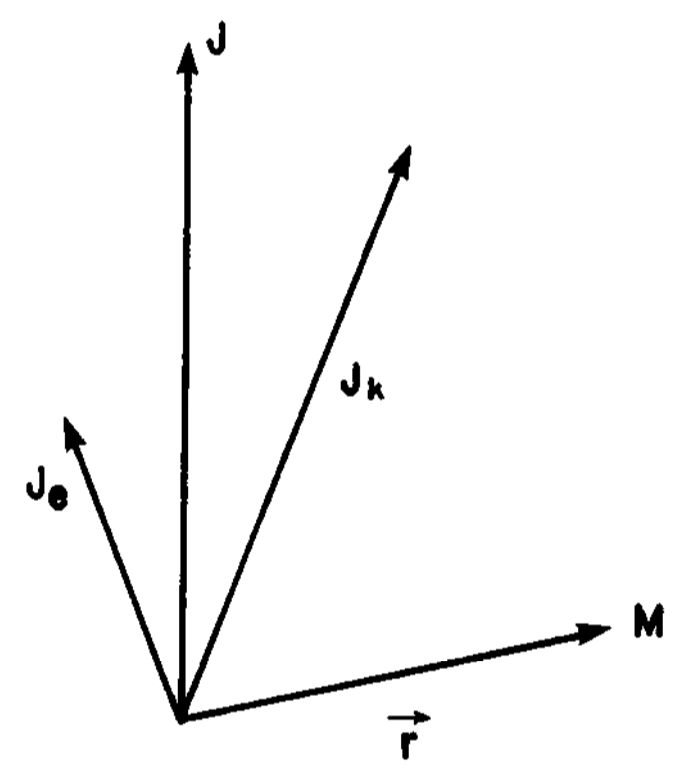
\includegraphics[width=150pt]{08-19200712-01}
	\end{center}
\end{figure}

Now $\vec{r} \perp \vec{J}_k$ (since $\vec{J}_k = 2M[\vec{r}\, \dot{\vec{r}}$) and $\vec{r} \perp \vec{J}_e$ (by assumption), so $\vec{r}\perp\vec{J}$ as well. But then the nuclear motion could only exist in a track around the invariable axis, so $J_e$ must also have this direction. Yet that cannot always be the case.

If these remarks have a big hole in them, please don't embarrass me in front of other people; but I think that it stands up well. — Indeed, the $\El{H}_2^+$ must be calculable ala Jakobi. Only working out every single possibility is so wearisome that without further clues, I don't want to poke around with it much.

Warmest greetings — faithfully yours,

Schr\"odinger

\end{letter}